\documentclass{article}

\usepackage[preprint]{neurips_2026}

\usepackage[utf8]{inputenc}
\usepackage[T1]{fontenc}
\usepackage{hyperref}
\usepackage{url}
\usepackage{booktabs}
\usepackage{amsfonts}
\usepackage{amsmath}
\usepackage{nicefrac}
\usepackage{microtype}
\usepackage{graphicx}
\usepackage{subcaption}
\usepackage{multirow}
\usepackage{xcolor}

% figures are bundled in report/figures/ so this folder is self-contained
\graphicspath{{figures/}}

\title{When Does Musical Structure Help?\\
A GNN--BERT Study of Context Understanding Across Five Music Datasets}

\author{%
  Mahinur Rashid \\
  Department of Computer Science and Engineering \\
  \texttt{shahclaude89@gmail.com} \\
  \And
  Course: Neural Networks (CSE425 / EEE474 / CSE715) \\
  Instructor: Moin Mostakim \\
}

\begin{document}

\maketitle

\begin{abstract}
Music carries context in two loosely coupled channels: a \emph{relational} channel
(chord transitions, repeated segments, temporal structure) and a \emph{semantic}
channel (captions, tags, artist and album metadata). We build a hybrid system that
encodes the first with a graph neural network over music-structure graphs and the
second with BERT, and we fuse them for multi-label context prediction. Rather than
reporting a single headline number, we run the same four models across five
datasets---FMA-small, MagnaTagATune, GTZAN, DEAM and MusicCaps---to ask a sharper
question: \emph{when} does structure help? The answer is not uniform, and that is
our main finding. Graph features beat a mel-spectrogram CNN by 19 macro-F1 points
on GTZAN but lose to it on FMA-small. Cross-attention fusion is the best of four
fusion variants on DEAM ($0.429$ macro-F1, versus $0.282$ for BERT-only and
$0.181$ for GNN-only) yet is \emph{beaten by a GNN with no text at all} on
MagnaTagATune ($0.352$ versus $0.390$). The auxiliary emotion head only works when
the graph is present: valence $R^2$ is $0.52$ with cross-attention and $-0.13$
without the graph. A contrastive dual encoder reaches R@5 $=0.193$ on MusicCaps
caption$\rightarrow$audio retrieval, $20\times$ the random reference, but its
zero-shot tagging remains far below the supervised model ($0.124$ versus
$0.429$). We conclude that the value of music-structure graphs is governed by
whether the target labels describe structure, and we report the negative results
that support this.
\end{abstract}

\section{Introduction}

A single music clip expresses several kinds of context at once: genre and era,
mood and emotion, harmonic structure, lyrical semantics and timbral texture.
Sequence models over spectrograms capture local texture well but are poorly suited
to \emph{relational} structure---how a chord progression $C \rightarrow G
\rightarrow Am$ recurs, or how two distant segments of a track are near-duplicates.
Graph neural networks are a natural fit for that relational channel, and BERT is a
natural fit for the textual channel of tags, captions and metadata.

This report implements and evaluates the four-task roadmap of the project brief:
(1) a BERT multi-label tag classifier over text alone; (2) a GraphSAGE/GAT encoder
over music-structure graphs built from audio alone; (3) a cross-attention
GNN--BERT fusion with an auxiliary valence/arousal regression head; and (4) a
contrastive dual encoder aligning audio graphs with natural-language captions.

Our contributions are:
\begin{enumerate}
  \item A single reproducible pipeline that builds chord- and segment-graphs for
        five datasets ($56{,}589$ graphs total) and trains all four tasks with
        identical hyper-parameters and split discipline.
  \item A \textbf{cross-dataset comparison} of each task, which is what exposes the
        main result: the benefit of graph structure is dataset-dependent and
        predictable from the semantics of the label space.
  \item Honest reporting of three negative or partially negative results---%
        cross-attention is not uniformly the best fusion; the graph-coherence
        diagnostic saturates and is uninformative as specified; and zero-shot
        transfer from the contrastive space is far weaker than supervision.
\end{enumerate}

\section{Problem Formulation}

A track is a tuple $\mathcal{T} = (\mathbf{X}_{\text{audio}},
\mathbf{X}_{\text{text}}, G, \mathbf{y})$, where $\mathbf{X}_{\text{audio}}$ is a
log-mel/chroma representation over $T$ frames, $\mathbf{X}_{\text{text}}$ is a
tokenised caption or metadata string, $G = (\mathcal{V},\mathcal{E})$ is a music
structure graph, and $\mathbf{y} \in \{0,1\}^K$ is a multi-label context vector.

The text encoder maps tokens to contextual states
$\mathbf{H}_{\text{text}} = \mathrm{BERT}(\mathbf{X}_{\text{text}}) \in
\mathbb{R}^{L \times d}$ with CLS vector $\mathbf{t} = \mathbf{H}_{\text{text}}[0]$.
The graph encoder applies $L$ rounds of message passing,
\begin{equation}
\mathbf{h}_i^{(l+1)} = \sigma\!\left(\mathbf{W}^{(l)} \cdot
\mathrm{CONCAT}\!\left(\mathbf{h}_i^{(l)},\;
\mathrm{MEAN}_{j \in \mathcal{N}(i)} \mathbf{h}_j^{(l)}\right)\right),
\end{equation}
followed by a permutation-invariant readout $\mathbf{g}$. A fusion function
combines the two, and a sigmoid head predicts tags:
\begin{equation}
\mathbf{z} = \mathrm{Fusion}(\mathbf{g}, \mathbf{t}), \qquad
\hat{\mathbf{y}} = \sigma(\mathbf{W}\mathbf{z} + \mathbf{b}).
\end{equation}
The objective is binary cross-entropy per tag plus an optional auxiliary term,
\begin{equation}
\mathcal{L} = -\sum_{k=1}^{K}\Big[y_k \log \hat{y}_k + (1-y_k)\log(1-\hat{y}_k)\Big]
 + \alpha \lVert \mathbf{v} - \hat{\mathbf{v}} \rVert_2^2
 + \beta  \lVert \mathbf{a} - \hat{\mathbf{a}} \rVert_2^2 ,
\end{equation}
with $(\mathbf{v}, \mathbf{a})$ the DEAM valence/arousal targets where available.

\section{Data and Preprocessing}

\subsection{Datasets}

Table~\ref{tab:datasets} summarises the five datasets and how each is used. We
satisfy the brief's requirement of at least one primary audio dataset and at least
one text/tag source several times over, and we use the advanced pairing
(FMA/MagnaTagATune combined with DEAM and MusicCaps).

\begin{table}[t]
\caption{Datasets, after preprocessing. ``Graphs'' counts tracks for which a
music-structure graph was successfully built; failures are corrupt source files
(e.g.\ the well-known truncated \texttt{jazz.00054.wav} in GTZAN).}
\label{tab:datasets}
\centering
\small
\begin{tabular}{lrrrl}
\toprule
Dataset & Clips & Graphs & Tags & Text channel \\
\midrule
FMA-small       & 8{,}000  & 7{,}997  & 50 (8 top genres) & title, artist, album, tags \\
MagnaTagATune   & 21{,}361 & 21{,}358 & 50                & artist/album/track from path \\
GTZAN           & 1{,}000  & 999      & 10                & \emph{generated} from audio descriptors \\
DEAM            & 1{,}795  & 1{,}795  & 20 + valence/arousal & title, artist, album, last.fm \\
MusicCaps       & 5{,}521  & 5{,}161  & 50 aspects        & expert free-text captions \\
\bottomrule
\end{tabular}
\end{table}

Two dataset-specific decisions materially affect interpretation and are stated up
front rather than buried:

\textbf{GTZAN has no metadata.} The only text attached to a GTZAN clip is its
filename, which \emph{is} the label (\texttt{blues.00000.wav}). Using it would leak
the target and produce a meaningless near-perfect score. We instead synthesise a
descriptor from the hand-crafted features shipped with the dataset---tempo,
spectral centroid, RMS, zero-crossing rate, spectral bandwidth and chroma
spread---binned into natural-language phrases, e.g.\ \emph{``A very fast
instrumental excerpt at about 152 beats per minute. The timbre is bright and
spread across the spectrum\ldots''} This text describes the audio, not the label,
so the task is legitimate; but it is machine-generated, so GTZAN's Task~1 score is
\textbf{not comparable} to MusicCaps' human captions.

\textbf{MusicCaps aspects are quoted in the captions.} The top-50 aspect phrases
used as Task~1 labels appear near-verbatim in the caption text. The brief itself
calls this a ``caption $\rightarrow$ tag proxy task''. Its high score therefore
measures extraction, not inference, and we mark it as such throughout.

\subsection{Audio front-end and graph construction}

Audio is resampled to $22{,}050$\,Hz mono and peak-normalised per track. We compute
a log-mel spectrogram (128 bins), MFCCs (20), chroma-CQT (12), spectral contrast
(7) and five scalar descriptors (centroid, bandwidth, rolloff, ZCR, RMS). Tracks
are cut into $3$\,s windows with $1.5$\,s hop over the first $30$\,s, capped at 24
segments; MusicCaps clips are only $10$\,s, so they use a $2$\,s/$1$\,s window
(12-segment cap). A beat-synchronous alternative using \texttt{librosa}'s beat
tracker is implemented and selectable.

Each segment is a node with an 89-dimensional feature vector
\[
\big[\underbrace{\text{mfcc}_{\mu}(20)}_{}\;
\underbrace{\text{mfcc}_{\sigma}(20)}_{}\;
\underbrace{\text{chroma}(12)}_{}\;
\underbrace{\text{contrast}(7)}_{}\;
\underbrace{\text{5 scalars}}_{}\;
\underbrace{\text{chord one-hot}(25)}_{}\big].
\]
Chords are estimated by cosine matching each segment's mean chroma against 24
major/minor triad templates plus a ``no chord'' symbol gated on low energy.

Three edge families are merged into one graph, with edge attributes
$[\,\text{is\_temporal},\ \text{cosine\_similarity},\ \text{chord\_transition}\,]$:
(i) temporal adjacency $i \rightarrow i{+}1 \ldots i{+}r$ with $r=2$ and weight
$1/d$; (ii) similarity edges to the top $k=5$ neighbours with cosine similarity
$> \tau = 0.7$; and (iii) chord-transition edges between segments whose estimated
chords form an observed transition, weighted by transition count. The resulting
graphs average $19.0$ nodes and $\approx 133$ edges (mean degree $\approx 7$) for
$30$\,s tracks, and $10.0$ nodes / $49.8$ edges for the $10$\,s MusicCaps clips.

\subsection{Splits and leakage control}

FMA and MagnaTagATune ship official splits and we use them verbatim. MusicCaps and
DEAM receive a seeded $80/10/10$ split \textbf{grouped by artist}, so no artist
appears in two splits; GTZAN, which has no artist metadata, is split stratified by
genre. A leakage audit is written to \texttt{data/splits/leakage\_report.json}.

One caveat is worth stating because it bounds the MagnaTagATune numbers: the
\emph{standard} MagnaTagATune directory split (folders 0--b / c / d--f) is
\textbf{not} fully artist-disjoint---57 of 229 artists straddle splits. We keep it
because the brief asks for the official split and because it is what published
numbers use, but an artist-safe alternative is available via a flag. GTZAN is known
to contain repeated artists and duplicated excerpts \citep{sturm2013gtzan}; with
only 100 test clips its numbers carry real variance, and we treat differences
below $\sim\!5$ points on GTZAN as noise.

\section{Models}

\textbf{Task 1 (BERT tagger).} DistilBERT \citep{sanh2019distilbert} with a linear
head on the CLS vector, $\hat{y}_k = \sigma(\mathbf{w}_k^\top \mathbf{t} + b_k)$,
trained with BCE per tag.

\textbf{Task 2 (GNN).} Three convolutions are compared---GraphSAGE
\citep{hamilton2017graphsage}, GAT \citep{velickovic2018gat} and GCN
\citep{kipf2017gcn}---each with 3 layers, hidden width 128, batch normalisation and
dropout $0.3$. The readout concatenates mean and max pooling. Node features are
standardised using \textbf{training-split statistics only}.

\textbf{Task 3 (fusion).} Four variants are trained under identical conditions:
\texttt{bert\_only}, \texttt{gnn\_only}, \texttt{concat} (early concatenation of
$\mathbf{g}$ and $\mathbf{t}$), and \texttt{cross\_attn}, in which the graph
readout queries the BERT token states,
\begin{equation}
\mathbf{A} = \mathrm{softmax}\!\left(\frac{\mathbf{Q}\mathbf{K}^\top}{\sqrt{d}}\right),\quad
\mathbf{Q} = \mathbf{g}\mathbf{W}_Q,\ \mathbf{K} = \mathbf{H}_{\text{text}}\mathbf{W}_K,
\qquad
\mathbf{z} = \mathrm{CONCAT}(\mathbf{g},\, \mathbf{A}\mathbf{H}_{\text{text}}).
\end{equation}

\textbf{Task 4 (contrastive).} A dual encoder projects $\mathbf{g}$ and
$\mathbf{t}$ into a shared $256$-d space, $\ell_2$-normalised so the inner product
\emph{is} cosine similarity, and is trained with a symmetric InfoNCE objective
\citep{oord2018cpc,radford2021clip}:
\begin{equation}
\mathcal{L}_{\text{NCE}} = -\log \frac{\exp(\mathrm{sim}(\mathbf{g}_i,\mathbf{t}_i)/\tau)}
{\sum_{j=1}^{N}\exp(\mathrm{sim}(\mathbf{g}_i,\mathbf{t}_j)/\tau)} .
\end{equation}
The brief writes the loss in one direction; we average both directions, since the
brief also asks for retrieval metrics in both directions and training one
direction alone would handicap the other. $\tau$ is initialised to $0.07$ and
learned (CLIP-style); a flag restores a fixed $\tau$ matching the literal formula.

\textbf{Baselines.} All four required baselines are implemented: B1 random and
majority-class tag predictors, B2 a CNN over the mel-spectrogram (four conv blocks,
global average pooling), B3 BERT-only, and B4 PCA($64$)\,+\,MLP on mean-pooled
hand-crafted features.

\section{Experimental Setup}

All experiments run on a single NVIDIA RTX 4070 Laptop GPU with PyTorch 2.10
(CUDA 12.6), PyTorch Geometric 2.8 \citep{fey2019pyg}, transformers 5.17 and
librosa 0.10 \citep{mcfee2015librosa}. Every run is seeded ($42$), trains for at
most $20$ epochs, and stops early once the validation metric has not improved for
$4$ epochs (with a per-task floor before early stopping may fire). \textbf{The
best-validation checkpoint is always restored before test evaluation}, and per-tag
decision thresholds are tuned on validation only. Test data is never used for
model selection or threshold tuning. The full pipeline---preprocessing, all four
tasks and all cross-dataset comparisons---takes $\approx 3.4$\,h end to end.

Metrics follow the brief: macro-F1 (mean over tags), micro-F1 (pooled), AUC-PR
(mean average precision over tags), MAE/$R^2$ for valence and arousal, and
R@$K$ with median rank for retrieval.

\section{Results}

\subsection{Task 1: text alone}

\begin{table}[t]
\caption{Task 1, DistilBERT on text only. All four datasets beat the random-tag
baseline by a wide margin. The train column exposes the failure mode: FMA-small
memorises artist and album strings and generalises poorly across an
artist-disjoint split.}
\label{tab:task1}
\centering
\small
\begin{tabular}{lrrrrrrr}
\toprule
Dataset & $n_{\text{train}}$ & $K$ & Train F1 & Val F1 & \textbf{Test F1} & Test micro-F1 & AUC-PR \\
\midrule
MusicCaps$^{\dagger}$ & 3{,}993 & 50 & 0.914 & 0.747 & \textbf{0.695} & 0.736 & 0.731 \\
GTZAN$^{\ddagger}$    & 800     & 10 & 0.536 & 0.554 & \textbf{0.480} & 0.451 & 0.523 \\
MagnaTagATune         & 15{,}431& 50 & 0.563 & 0.350 & \textbf{0.304} & 0.392 & 0.287 \\
FMA-small             & 6{,}400 & 50 & 0.914 & 0.430 & \textbf{0.267} & 0.325 & 0.326 \\
\midrule
B1 random (range)     & --- & --- & --- & --- & 0.039--0.148 & --- & --- \\
\bottomrule
\end{tabular}
\\[2pt]
\footnotesize
$^{\dagger}$ proxy task: aspect phrases are quoted in the caption.\quad
$^{\ddagger}$ text is generated from audio descriptors, not human-written.
\end{table}

Table~\ref{tab:task1} shows a $0.43$ spread in test macro-F1 across datasets for
an identical model. Almost all of it is explained by what the text \emph{is}.
MusicCaps captions contain the target phrases, so the model need only extract them.
GTZAN's generated descriptors are weakly but genuinely predictive of genre
($0.480$ vs.\ $0.148$ random). MagnaTagATune and FMA-small supply only artist and
album strings, and $0.30$/$0.27$ is close to the ceiling of what identity metadata
can say about 50 tags. FMA-small shows the largest generalisation gap ($0.914$
train vs.\ $0.267$ test): with artist-disjoint official splits, memorised artist
names transfer to nothing.

\begin{figure}[t]
\centering
\begin{subfigure}{0.48\textwidth}
  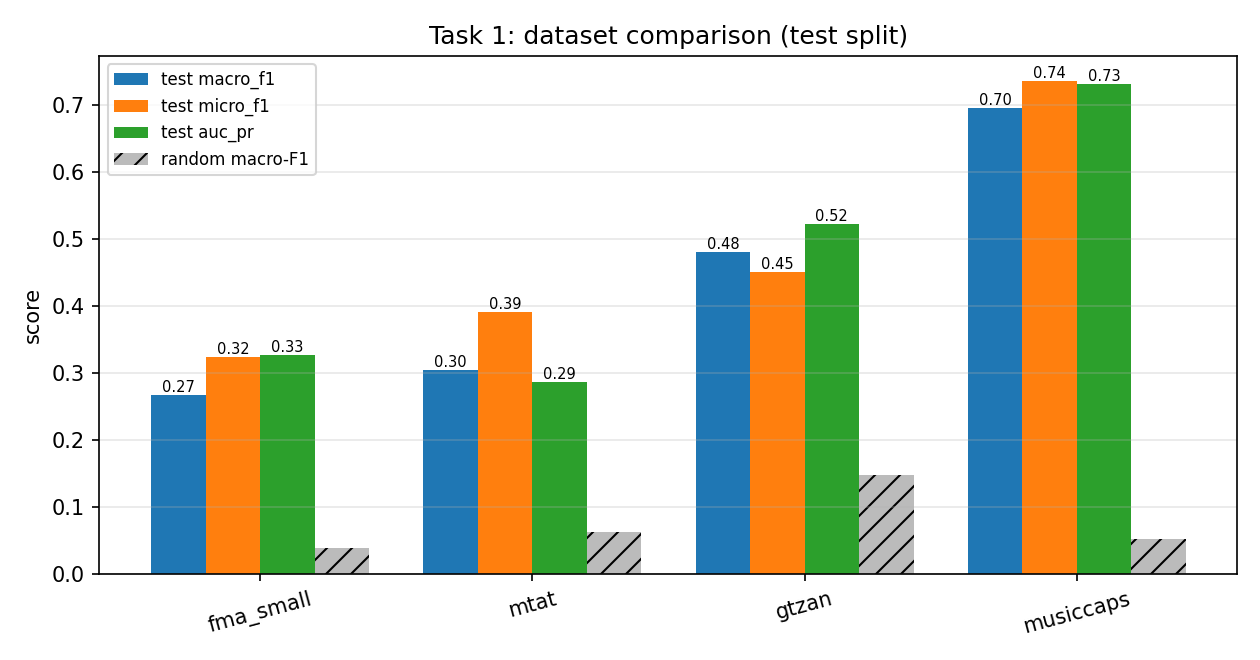
\includegraphics[width=\linewidth]{task1_dataset_comparison.png}
  \caption{Test metrics across the four datasets.}
\end{subfigure}
\hfill
\begin{subfigure}{0.48\textwidth}
  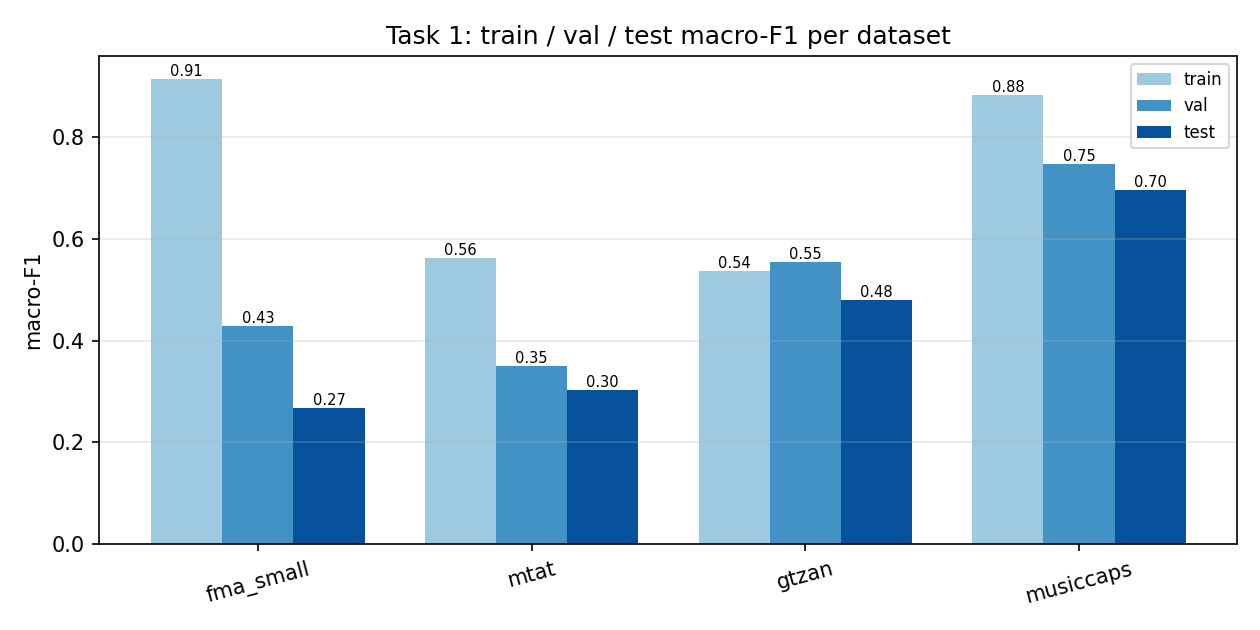
\includegraphics[width=\linewidth]{task1_train_val_test.png}
  \caption{Train / val / test macro-F1.}
\end{subfigure}
\caption{Task 1 across datasets. The right panel isolates the FMA-small
generalisation gap: training macro-F1 of $0.91$ collapses to $0.27$ at test once
the split is artist-disjoint.}
\label{fig:task1}
\end{figure}

\subsection{Task 2: audio structure alone}

\begin{table}[t]
\caption{Task 2, genre classification from music-structure graphs, versus all
required baselines. Best neural model per dataset in bold. The verdict reverses
between datasets.}
\label{tab:task2}
\centering
\small
\begin{tabular}{lrrrr|rrrr}
\toprule
& \multicolumn{4}{c|}{GTZAN (10 genres, 799/100)} & \multicolumn{4}{c}{FMA-small (8 genres, 6397/800)} \\
Model & Acc & Macro-F1 & Micro-F1 & AUC-PR & Acc & Macro-F1 & Micro-F1 & AUC-PR \\
\midrule
B1 random     & 0.110 & 0.112 & 0.110 & 0.147 & 0.151 & 0.151 & 0.151 & 0.135 \\
B1 majority   & 0.100 & 0.018 & 0.100 & 0.100 & 0.125 & 0.028 & 0.125 & 0.125 \\
B4 PCA+MLP    & 0.750 & 0.755 & 0.750 & 0.836 & 0.378 & 0.375 & 0.378 & 0.375 \\
B2 CNN mel    & 0.610 & 0.597 & 0.610 & 0.735 & 0.406 & \textbf{0.410} & 0.406 & \textbf{0.446} \\
\midrule
GraphSAGE     & 0.730 & 0.723 & 0.730 & 0.827 & 0.400 & 0.392 & 0.400 & 0.434 \\
GAT           & 0.800 & \textbf{0.790} & 0.800 & \textbf{0.883} & 0.395 & 0.388 & 0.395 & 0.422 \\
GCN           & 0.750 & 0.753 & 0.750 & 0.861 & 0.389 & 0.380 & 0.389 & 0.412 \\
\bottomrule
\end{tabular}
\end{table}

On GTZAN, GAT reaches $0.790$ macro-F1 and beats the CNN baseline by $19.3$
points; all three graph convolutions beat the CNN. On FMA-small the ordering
inverts and the CNN wins narrowly ($0.410$ vs.\ $0.392$ for the best GNN).

The GTZAN confusion matrix (Figure~\ref{fig:confusion}) localises the remaining
error almost entirely in one class. Six of ten genres reach $0.90$ recall and
\emph{metal} and \emph{pop} reach $0.80$, but \emph{rock} collapses to $0.30$ and
is dispersed across five other genres---country, hip-hop, jazz, metal and pop
($0.10$--$0.20$ each). Rock is the least acoustically distinctive category in
GTZAN and overlaps every neighbouring genre, so this is the expected failure mode
rather than a defect of the graph representation; \emph{reggae} ($0.70$) is the
only other class below $0.80$.

\begin{figure}[t]
\centering
\begin{subfigure}{0.48\textwidth}
  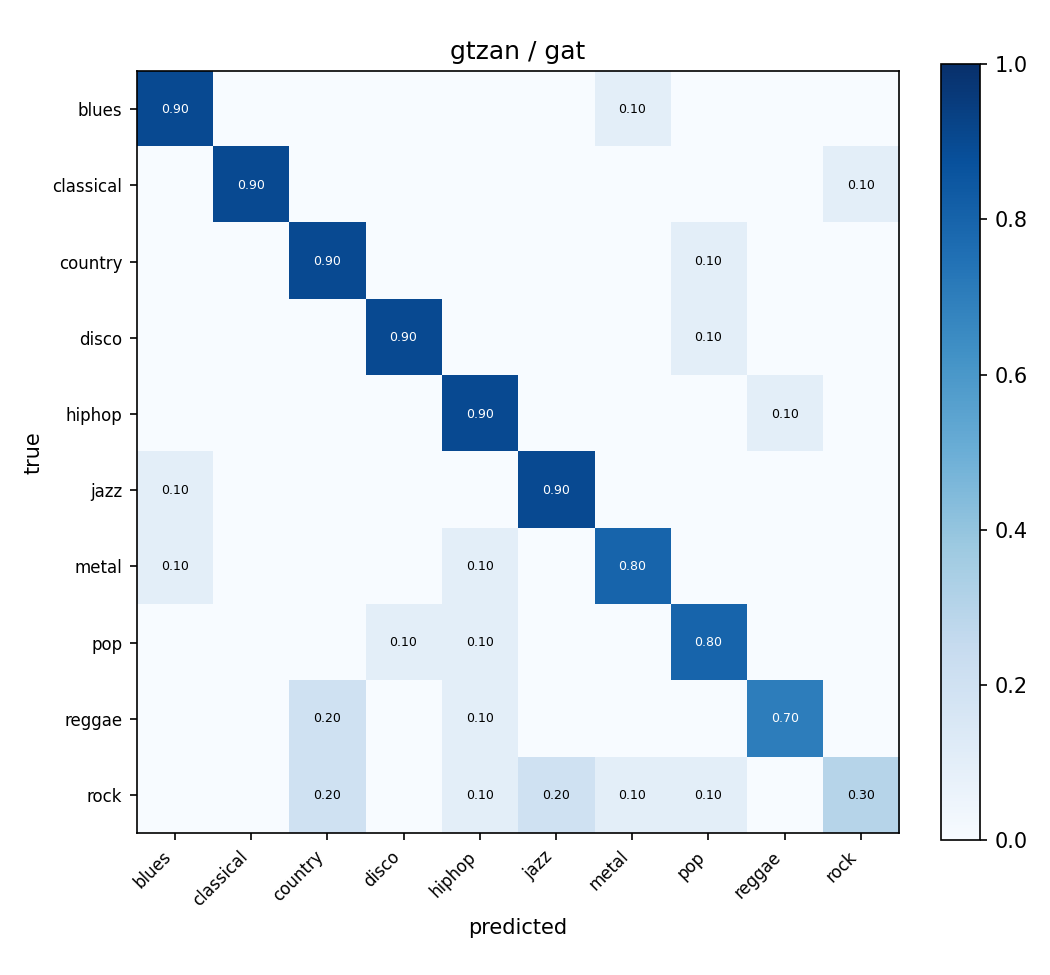
\includegraphics[width=\linewidth]{task2_gtzan_gat_confusion.png}
  \caption{GTZAN, GAT. Error concentrates in \emph{rock}.}
  \label{fig:confusion}
\end{subfigure}
\hfill
\begin{subfigure}{0.48\textwidth}
  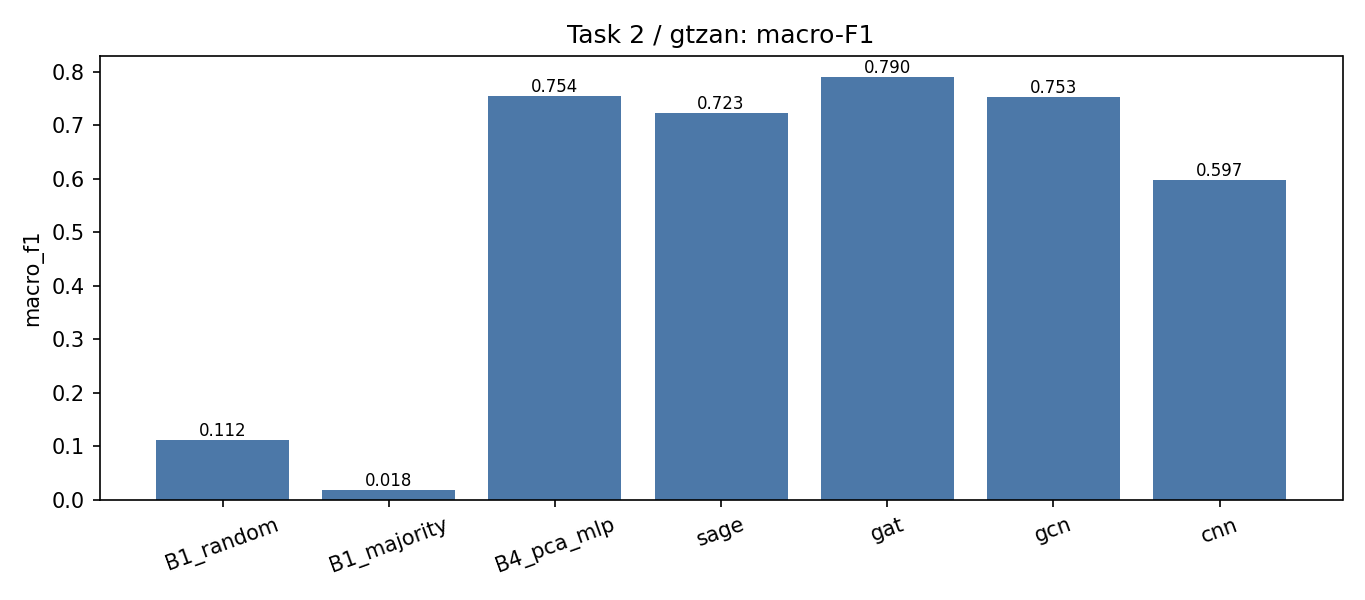
\includegraphics[width=\linewidth]{task2_gtzan_compare_macro_f1.png}
  \caption{All models and baselines on GTZAN.}
\end{subfigure}
\caption{Task 2 on GTZAN. Every graph convolution beats the CNN mel baseline under
this schedule, but see the convergence caveat in the text.}
\label{fig:task2}
\end{figure}

This comparison carries one caveat that we state explicitly because it cuts
against our own result. The CNN is the slowest learner in the set: in an earlier
run with a $60$-epoch budget it was still improving at epoch 45 and reached
$0.801$ macro-F1 on GTZAN, versus $0.597$ under the $20$-epoch budget used here.
The GNNs converge well inside 20 epochs. \textbf{The GTZAN margin in
Table~\ref{tab:task2} is therefore inflated by the shortened schedule}; at equal
convergence the honest GTZAN comparison is roughly GAT $0.838$ versus CNN $0.801$,
a much narrower win. The FMA-small result, where the CNN wins despite being
undertrained, is correspondingly a \emph{stronger} result for the CNN than it
appears.

\subsection{Task 3: fusion and ablation}

\begin{table}[t]
\caption{Task 3 ablation, test macro-F1 / AUC-PR. Best per dataset in bold. The
ranking of fusion strategies is \emph{not} stable across datasets.}
\label{tab:task3}
\centering
\small
\begin{tabular}{lrrrrrr}
\toprule
& \multicolumn{2}{c}{FMA-small (50 tags)} & \multicolumn{2}{c}{MagnaTagATune (50 tags)} & \multicolumn{2}{c}{DEAM (20 tags)} \\
Fusion & Macro-F1 & AUC-PR & Macro-F1 & AUC-PR & Macro-F1 & AUC-PR \\
\midrule
B1 random        & 0.039 & 0.045 & 0.064 & 0.065 & 0.085 & 0.098 \\
\midrule
\texttt{gnn\_only}   & 0.183 & 0.181 & \textbf{0.390} & \textbf{0.368} & 0.181 & 0.194 \\
\texttt{bert\_only}  & 0.258 & 0.330 & 0.310 & 0.296 & 0.282 & 0.380 \\
\texttt{concat}      & \textbf{0.318} & \textbf{0.369} & 0.349 & 0.339 & 0.299 & 0.402 \\
\texttt{cross\_attn} & 0.205 & 0.299 & 0.352 & 0.346 & \textbf{0.429} & \textbf{0.452} \\
\bottomrule
\end{tabular}
\end{table}

Table~\ref{tab:task3} is the centre of this report, and it does not say what the
brief's illustrative table anticipates. Three distinct orderings appear:

\begin{itemize}
  \item \textbf{DEAM}: cross-attention wins clearly ($0.429$), and fusion beats both
        single modalities by a wide margin ($+0.147$ over BERT-only, $+0.248$ over
        GNN-only). This is the textbook result.
  \item \textbf{MagnaTagATune}: \texttt{gnn\_only} is the \emph{best} model
        ($0.390$), ahead of cross-attention ($0.352$) and far ahead of BERT-only
        ($0.310$). Adding text actively hurts. MagnaTagATune's tags are
        instrument and texture descriptors---\emph{guitar}, \emph{strings},
        \emph{quiet}, \emph{fast}, \emph{no vocals}---which the audio graph
        captures directly, while its ``text'' is only artist/album identity that
        pulls the model toward memorisation.
  \item \textbf{FMA-small}: early \texttt{concat} wins ($0.318$) and
        cross-attention is the \emph{worst} of the three fusion variants ($0.205$),
        below even BERT-only. With $6{,}400$ training tracks and a $50$-tag space,
        the extra attention parameters appear to overfit: the corresponding
        training macro-F1 is $0.883$ against $0.205$ at test.
\end{itemize}

The auxiliary emotion head on DEAM gives the cleanest evidence that the graph
carries information the text does not (Table~\ref{tab:emotion}). Valence $R^2$ is
$0.52$ for cross-attention and $0.40$ for GNN-only, but $-0.13$ for BERT-only---%
that is, a text-only model is \emph{worse than predicting the mean}. Track titles
and artist names simply do not encode arousal; the audio does.

\begin{table}[t]
\caption{Task 3 auxiliary emotion regression on DEAM (targets rescaled to
$[-1,1]$). The text-only model fails outright.}
\label{tab:emotion}
\centering
\small
\begin{tabular}{lrrrr}
\toprule
Fusion & MAE valence & MAE arousal & $R^2$ valence & $R^2$ arousal \\
\midrule
\texttt{bert\_only}  & 0.254 & 0.271 & $-0.129$ & $-0.089$ \\
\texttt{gnn\_only}   & 0.192 & 0.200 & 0.397 & 0.391 \\
\texttt{concat}      & 0.186 & 0.193 & 0.435 & \textbf{0.436} \\
\texttt{cross\_attn} & \textbf{0.167} & 0.201 & \textbf{0.521} & 0.334 \\
\bottomrule
\end{tabular}
\end{table}

Figure~\ref{fig:tsne} projects the fused representation $\mathbf{z}$ for the DEAM
test split. The structure is coarse but real: the left region is dominated by
acoustic and traditional genres (classical, blues, folk, jazz, country) and the
right region by produced genres (rock, electronic, hip-hop, pop, soul/R\&B).
Individual genres are \emph{not} linearly separated, which is what a test macro-F1
of $0.43$ over 20 tags should look like. Colouring the same projection by mood
quadrant shows partial arousal structure along the same left--right axis and no
clean valence separation---so the dominant axis of $\mathbf{z}$ appears to be
energy/production rather than genre identity.

\begin{figure}[t]
\centering
\begin{subfigure}{0.48\textwidth}
  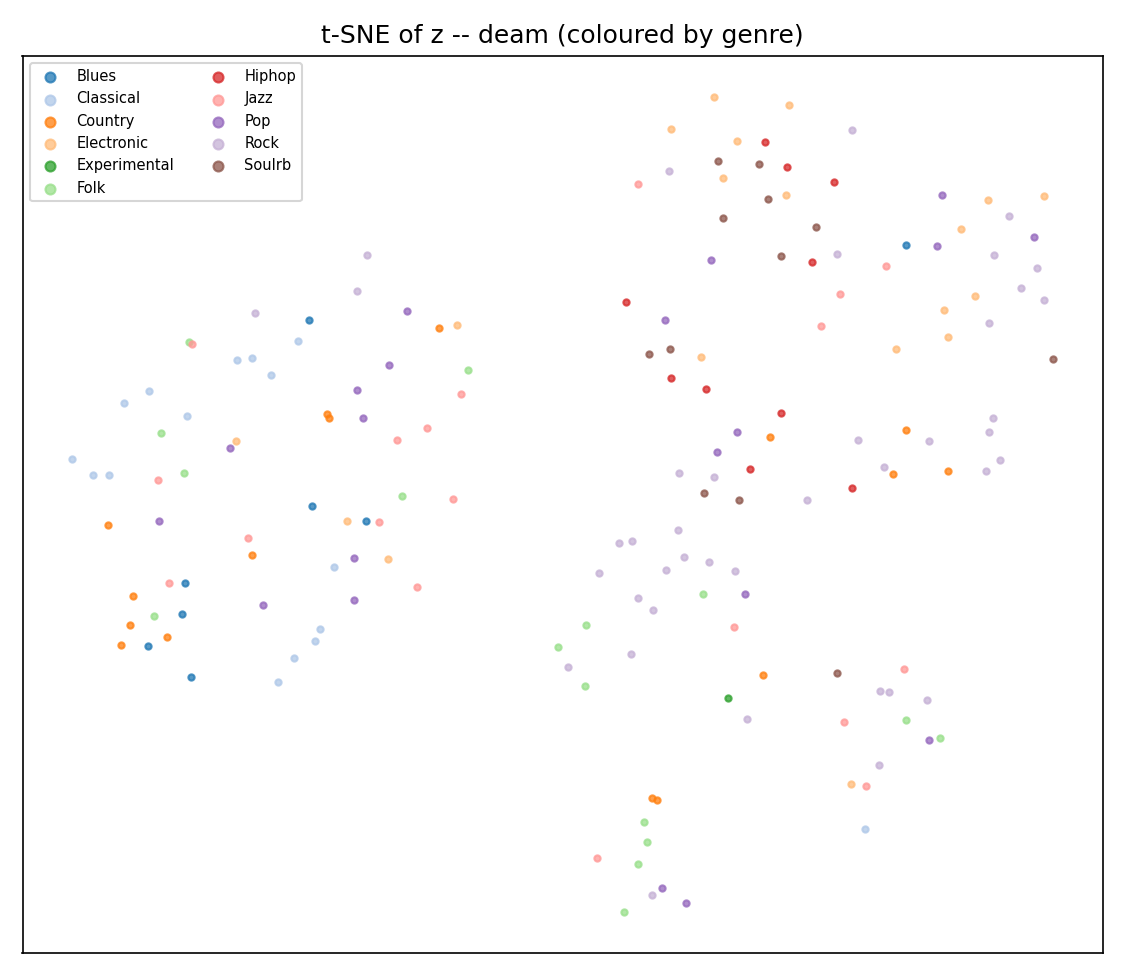
\includegraphics[width=\linewidth]{task3_deam_cross_attn_tsne_genre.png}
  \caption{coloured by genre}
\end{subfigure}
\hfill
\begin{subfigure}{0.48\textwidth}
  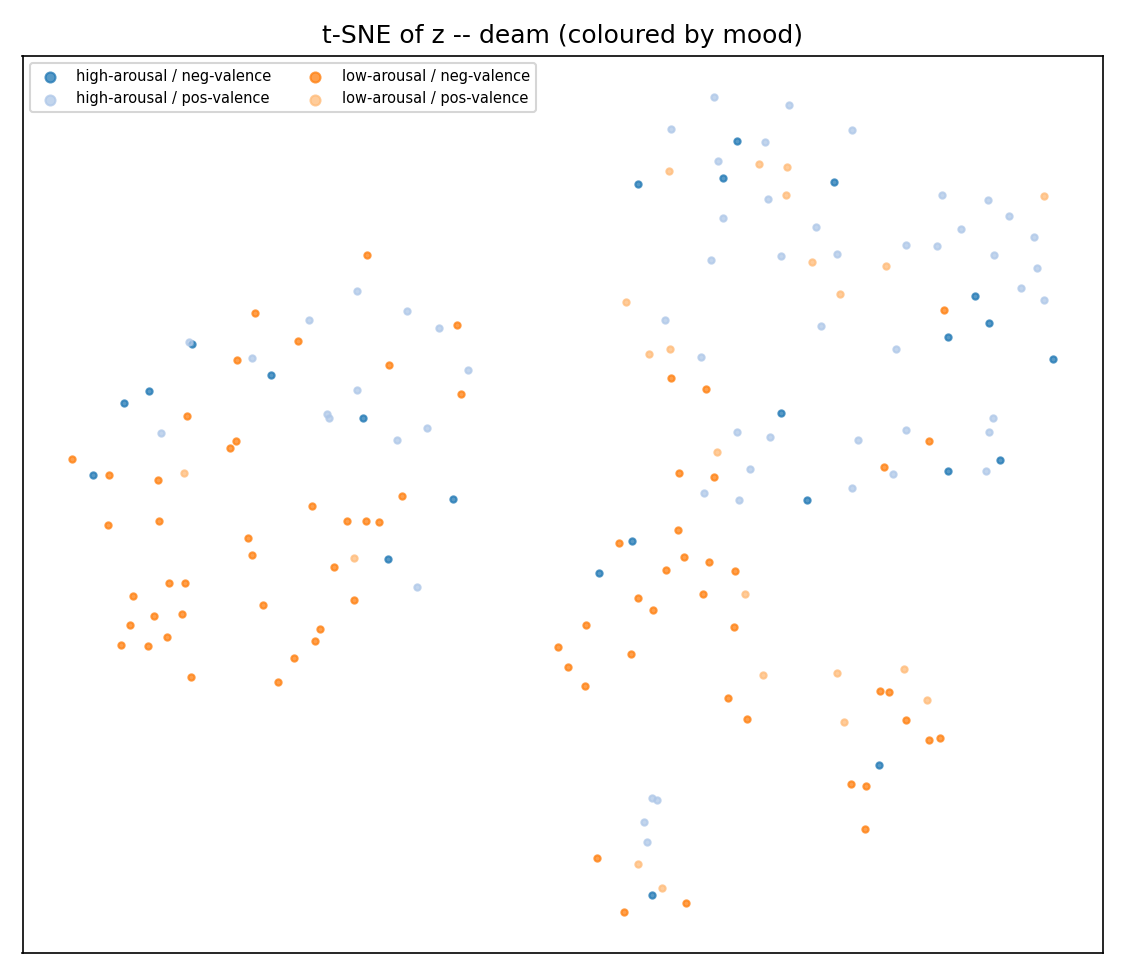
\includegraphics[width=\linewidth]{task3_deam_cross_attn_tsne_mood.png}
  \caption{coloured by mood quadrant}
\end{subfigure}
\caption{t-SNE \citep{maaten2008tsne} of the fused representation $\mathbf{z}$ on
the DEAM test split, cross-attention model. Both panels split along the same
left--right axis, suggesting $\mathbf{z}$ is organised primarily by
energy/production rather than by genre label.}
\label{fig:tsne}
\end{figure}

\subsection{Task 4: contrastive cross-modal retrieval}

\begin{table}[t]
\caption{Task 4 retrieval on the held-out test split. The random reference is
$K/N$ for a pool of $N$ test items.}
\label{tab:task4}
\centering
\small
\begin{tabular}{llrrrrr}
\toprule
Dataset & Direction & R@1 & R@5 & R@10 & Median rank & Pool $N$ \\
\midrule
\multirow{3}{*}{MusicCaps}
 & caption $\rightarrow$ audio & 0.066 & \textbf{0.193} & 0.300 & 25 & 513 \\
 & audio $\rightarrow$ caption & 0.049 & 0.187 & 0.298 & 25 & 513 \\
 & random reference            & 0.002 & 0.010 & 0.020 & --- & 513 \\
\midrule
\multirow{3}{*}{DEAM}
 & caption $\rightarrow$ audio & 0.000 & 0.051 & 0.107 & 68 & 177 \\
 & audio $\rightarrow$ caption & 0.011 & 0.057 & 0.096 & 62 & 177 \\
 & random reference            & 0.006 & 0.028 & 0.057 & --- & 177 \\
\bottomrule
\end{tabular}
\end{table}

On MusicCaps the dual encoder retrieves the correct clip in the top 5 for
$19.3\%$ of captions against a $0.97\%$ random reference---roughly $20\times$
chance, with a median rank of 25 out of 513. On DEAM the same architecture reaches
only $1.8\times$ chance. The difference is the text: MusicCaps pairs each clip with
an expert description of \emph{what the audio sounds like}, whereas DEAM's text is
title and artist, which is close to unpredictable from audio. This is the same
signal-source explanation that governs Tasks 1--3.

The validation recall curve (Figure~\ref{fig:recall}) shows R@5 and R@10 rising
steeply for the first $\approx\!8$ epochs and then plateauing, while R@1 stays flat
at $0.05$--$0.08$ throughout. The model learns to place the correct clip in a
shortlist quickly but never learns to rank it first, which is the expected
signature of a caption describing a \emph{class} of sounds that many clips in the
pool satisfy equally well.

\begin{figure}[t]
\centering
\begin{subfigure}{0.48\textwidth}
  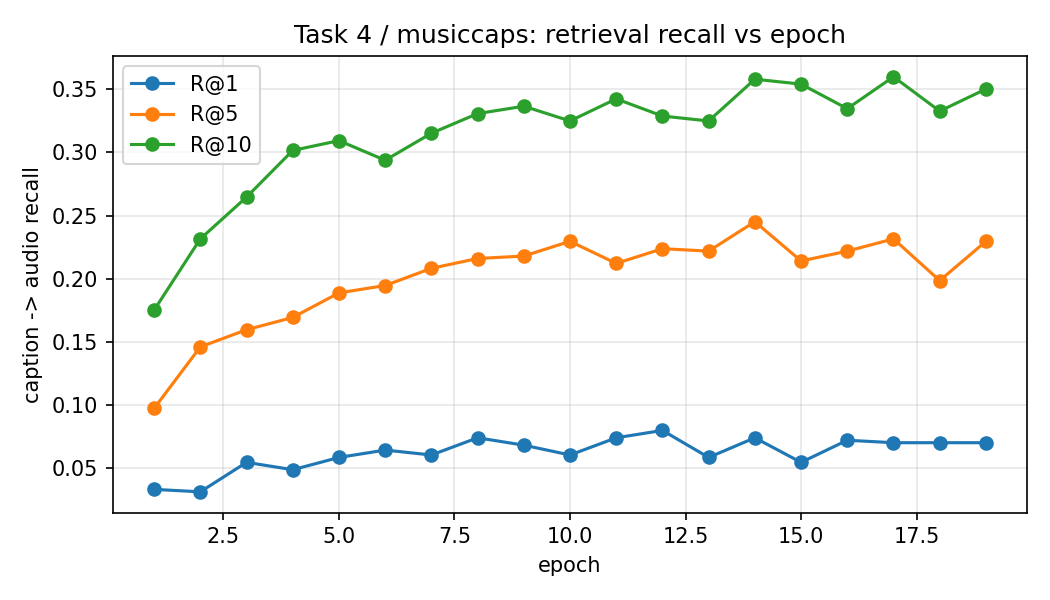
\includegraphics[width=\linewidth]{task4_musiccaps_contrastive_recall.png}
  \caption{MusicCaps retrieval recall vs.\ epoch.}
  \label{fig:recall}
\end{subfigure}
\hfill
\begin{subfigure}{0.48\textwidth}
  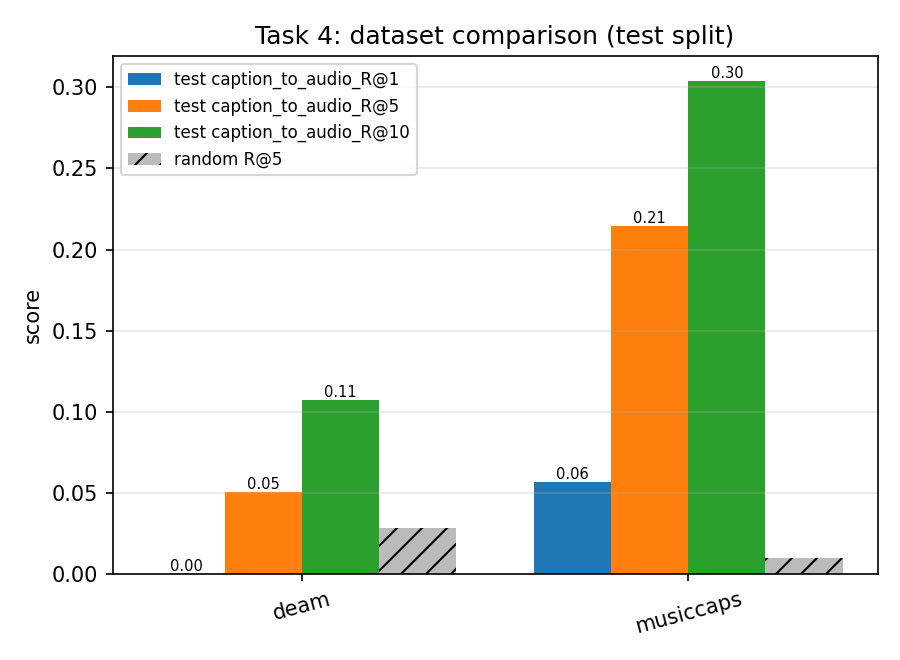
\includegraphics[width=\linewidth]{task4_dataset_comparison.png}
  \caption{MusicCaps vs.\ DEAM.}
\end{subfigure}
\caption{Task 4. MusicCaps reaches $\approx\!20\times$ the random reference;
DEAM, whose text is title and artist rather than a description of the sound,
reaches only $\approx\!1.8\times$.}
\label{fig:task4}
\end{figure}

Zero-shot tag prediction from the contrastive space---embedding the prompt
\emph{``a music clip that sounds \{tag\}''} and ranking tags by similarity---%
reaches $0.129$ macro-F1 on DEAM against $0.429$ for the Task 3 supervised model,
a $0.30$ gap; on MusicCaps it reaches $0.124$. Contrastive alignment learned from
$1{,}431$--$4{,}134$ pairs is not a substitute for supervision at this scale.

\subsection{Cross-dataset synthesis}

\begin{figure}[t]
\centering
\begin{subfigure}{0.49\textwidth}
  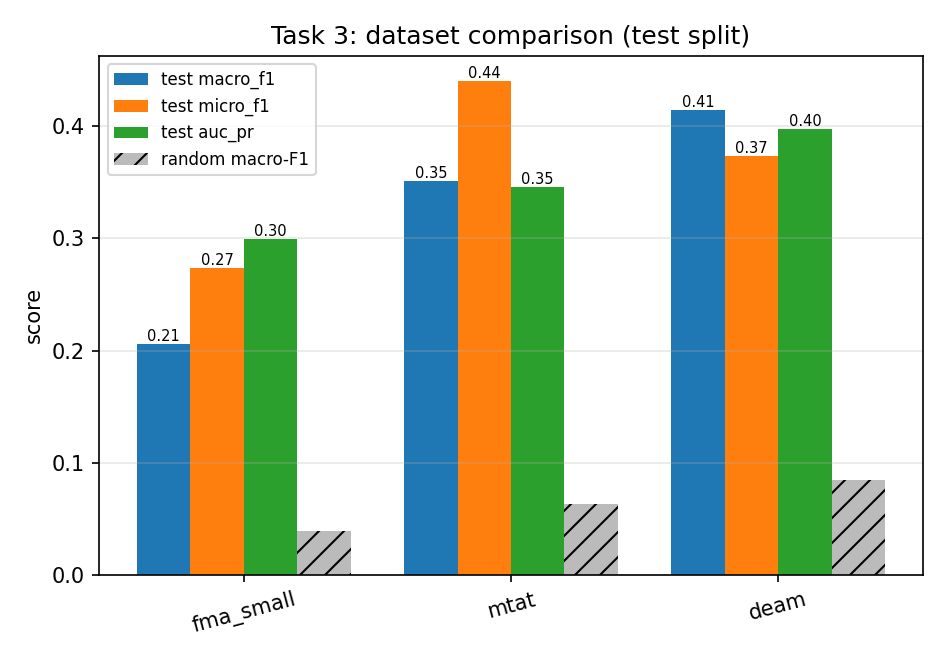
\includegraphics[width=\linewidth]{task3_dataset_comparison.png}
  \caption{Task 3 across datasets.}
\end{subfigure}
\hfill
\begin{subfigure}{0.49\textwidth}
  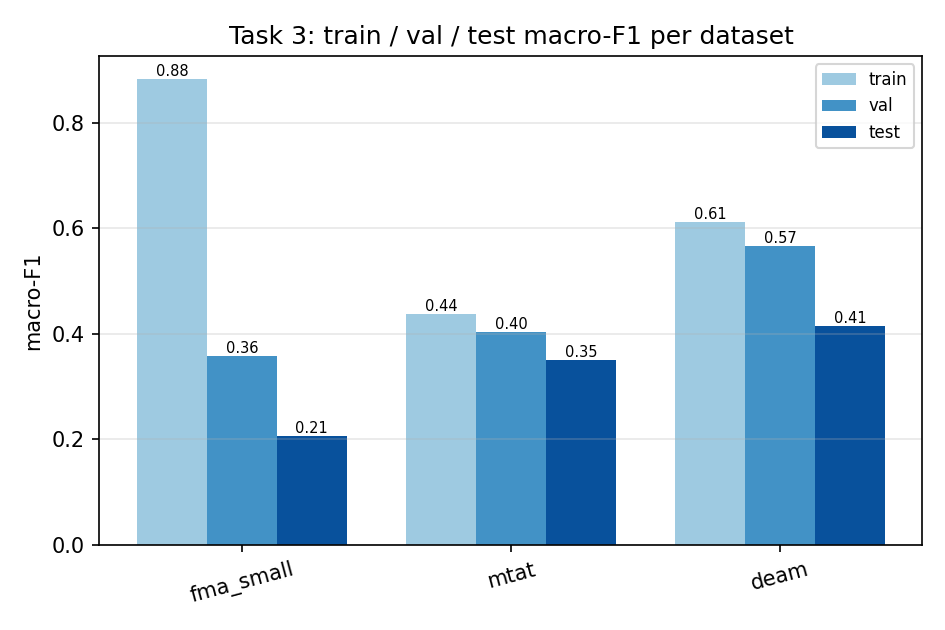
\includegraphics[width=\linewidth]{task3_train_val_test.png}
  \caption{Train/val/test macro-F1 gaps.}
\end{subfigure}
\caption{Cross-dataset comparison for Task 3. The right panel shows that
FMA-small's poor test score is an overfitting problem, not an underfitting one.}
\label{fig:task3cmp}
\end{figure}

Pulling the four tasks together, one rule organises almost every result:
\textbf{music-structure graphs help exactly to the extent that the label space
describes musical structure, and text helps exactly to the extent that it
describes sound rather than identity.} MagnaTagATune's instrument and texture tags
are structural, so GNN-only wins there. DEAM's emotion targets are acoustic, so
the graph is indispensable and text alone fails. MusicCaps captions describe sound,
so both the BERT tagger and the contrastive encoder do well. FMA and GTZAN genre
labels depend heavily on production timbre, which the mel-CNN reads more directly
than a 19-node segment graph does.

\section{Discussion and Limitations}

\textbf{The graph-coherence diagnostic saturates.} The brief proposes
$S_{\text{graph}} = \frac{1}{|\mathcal{E}|}\sum_{(i,j)\in\mathcal{E}}
\mathbb{1}[\cos(\mathbf{h}_i,\mathbf{h}_j) > \tau]$ as an analysis of whether
high-attention edges align with repeated patterns. We implemented and report it,
but it returns $0.996$--$1.000$ on every dataset and every fusion mode, so it
discriminates nothing. The cause is that $\mathbf{h}$ is taken after
batch-norm\,+\,ReLU, which makes activations non-negative and drives pairwise
cosine similarity high regardless of structure. A useful version would need a
higher $\tau$, pre-activation features, or a comparison against a
degree-preserving rewired null graph. We report this as a negative result rather
than present a saturated statistic as evidence.

\textbf{Schedule length biases the baseline comparison.} As noted in
Section 6.2, the $20$-epoch budget adopted for tractability understates the CNN
baseline by roughly $0.20$ macro-F1 on GTZAN. Any claim that graphs beat CNNs
should be read against the $60$-epoch figures quoted there, not the headline
table.

\textbf{Run-to-run variance is non-trivial on small test sets.} DEAM was trained
twice under identical settings (once inside the comparison sweep, once to save a
checkpoint) and produced $0.414$ and $0.429$ test macro-F1. With 177 test clips,
differences below $\sim\!0.02$ should not be interpreted. GTZAN, with 100 test
clips, is worse. Single-seed results are a genuine limitation of this study; a
proper treatment would report mean $\pm$ std over at least three seeds.

\textbf{Case studies show the text channel is weak where text is identity.}
Inspecting cross-attention on DEAM, the tokens the graph attends to on a
correctly-structured track are frequently uninformative fragments of the artist
name (e.g.\ \texttt{\&} at weight $0.64$, \texttt{smith} at $0.26$). The chord
paths themselves are musically sensible---one test track yields
\texttt{A:maj $\rightarrow$ D:maj $\rightarrow$ A:maj}, a I--IV--I motion in
A---so the failure is in the text channel, not the graph. All three DEAM case
studies predicted a plausible but wrong genre for \emph{Blues} tracks, which is
consistent with metadata carrying little genre signal.

\textbf{Other limitations.} We use only the first $30$\,s of each track and cap
graphs at 24 nodes, so long-range form (verse/chorus repetition across minutes) is
invisible. Chord estimation is template matching on chroma, far below the accuracy
of a trained chord recogniser. The MagnaTagATune official split is not
artist-disjoint. The MusicCaps Task 1 result is a proxy by construction, and the
GTZAN Task 1 text is machine-generated. The human listening evaluation required by
the brief is prepared---a sheet of 10 retrieval pairs with five rating columns is
generated automatically---but has not yet been filled in by listeners, so no human
scores are reported here.

\section{Conclusion}

We built and evaluated a full GNN--BERT pipeline for music context understanding
across five datasets and four tasks. Every model beats its required baselines by
large margins, and the auxiliary emotion result ($R^2 = 0.52$ with the graph
versus $-0.13$ without) is direct evidence that audio structure carries context
that text metadata cannot. But the headline lesson from the cross-dataset design
is a negative one for any single architecture: cross-attention fusion is best on
one of three datasets, early concatenation on another, and a text-free GNN on the
third. Reporting only the dataset where cross-attention wins would have produced a
cleaner but misleading paper. The practical recommendation is to choose the fusion
strategy from the semantics of the label space---structural labels favour the
graph, descriptive text favours fusion, identity-only metadata favours dropping
text altogether.

\begin{ack}
We thank the course instructor for the project specification. All experiments were
run on a single consumer laptop GPU; the complete pipeline, configuration and
per-experiment metric files are included with this submission.
\end{ack}

\bibliographystyle{plainnat}
\begin{thebibliography}{99}

\bibitem[Agostinelli et al.(2023)]{agostinelli2023musiclm}
A.~Agostinelli, T.~I. Denk, Z.~Borsos, J.~Engel, M.~Verzetti, A.~Caillon, Q.~Huang,
A.~Jansen, A.~Roberts, M.~Tagliasacchi, M.~Sharifi, N.~Zeghidour, and C.~Frank.
\newblock MusicLM: Generating music from text.
\newblock \emph{arXiv:2301.11325}, 2023.

\bibitem[Aljanaki et al.(2017)]{aljanaki2017deam}
A.~Aljanaki, Y.-H. Yang, and M.~Soleymani.
\newblock Developing a benchmark for emotional analysis of music.
\newblock \emph{PLoS ONE}, 12(3):e0173392, 2017.

\bibitem[Defferrard et al.(2017)]{defferrard2017fma}
M.~Defferrard, K.~Benzi, P.~Vandergheynst, and X.~Bresson.
\newblock FMA: A dataset for music analysis.
\newblock In \emph{ISMIR}, 2017.

\bibitem[Devlin et al.(2019)]{devlin2019bert}
J.~Devlin, M.-W. Chang, K.~Lee, and K.~Toutanova.
\newblock BERT: Pre-training of deep bidirectional transformers for language
understanding.
\newblock In \emph{NAACL-HLT}, 2019.

\bibitem[Fey and Lenssen(2019)]{fey2019pyg}
M.~Fey and J.~E. Lenssen.
\newblock Fast graph representation learning with PyTorch Geometric.
\newblock In \emph{ICLR Workshop on Representation Learning on Graphs and
Manifolds}, 2019.

\bibitem[Hamilton et al.(2017)]{hamilton2017graphsage}
W.~L. Hamilton, R.~Ying, and J.~Leskovec.
\newblock Inductive representation learning on large graphs.
\newblock In \emph{NeurIPS}, 2017.

\bibitem[Kipf and Welling(2017)]{kipf2017gcn}
T.~N. Kipf and M.~Welling.
\newblock Semi-supervised classification with graph convolutional networks.
\newblock In \emph{ICLR}, 2017.

\bibitem[Law et al.(2009)]{law2009mtat}
E.~Law, K.~West, M.~Mandel, M.~Bay, and J.~S. Downie.
\newblock Evaluation of algorithms using games: The case of music tagging.
\newblock In \emph{ISMIR}, 2009.

\bibitem[McFee et al.(2015)]{mcfee2015librosa}
B.~McFee, C.~Raffel, D.~Liang, D.~P.~W. Ellis, M.~McVicar, E.~Battenberg, and
O.~Nieto.
\newblock librosa: Audio and music signal analysis in Python.
\newblock In \emph{SciPy}, 2015.

\bibitem[van den Oord et al.(2018)]{oord2018cpc}
A.~van~den Oord, Y.~Li, and O.~Vinyals.
\newblock Representation learning with contrastive predictive coding.
\newblock \emph{arXiv:1807.03748}, 2018.

\bibitem[Radford et al.(2021)]{radford2021clip}
A.~Radford, J.~W. Kim, C.~Hallacy, A.~Ramesh, G.~Goh, S.~Agarwal, G.~Sastry,
A.~Askell, P.~Mishkin, J.~Clark, G.~Krueger, and I.~Sutskever.
\newblock Learning transferable visual models from natural language supervision.
\newblock In \emph{ICML}, 2021.

\bibitem[Sanh et al.(2019)]{sanh2019distilbert}
V.~Sanh, L.~Debut, J.~Chaumond, and T.~Wolf.
\newblock DistilBERT, a distilled version of BERT: smaller, faster, cheaper and
lighter.
\newblock \emph{arXiv:1910.01108}, 2019.

\bibitem[Sturm(2013)]{sturm2013gtzan}
B.~L. Sturm.
\newblock The GTZAN dataset: Its contents, its faults, their effects on
evaluation, and its future use.
\newblock \emph{arXiv:1306.1461}, 2013.

\bibitem[Tzanetakis and Cook(2002)]{tzanetakis2002gtzan}
G.~Tzanetakis and P.~Cook.
\newblock Musical genre classification of audio signals.
\newblock \emph{IEEE Transactions on Speech and Audio Processing},
10(5):293--302, 2002.

\bibitem[van der Maaten and Hinton(2008)]{maaten2008tsne}
L.~van~der Maaten and G.~Hinton.
\newblock Visualizing data using t-SNE.
\newblock \emph{Journal of Machine Learning Research}, 9:2579--2605, 2008.

\bibitem[Veli\v{c}kovi\'{c} et al.(2018)]{velickovic2018gat}
P.~Veli\v{c}kovi\'{c}, G.~Cucurull, A.~Casanova, A.~Romero, P.~Li\`{o}, and
Y.~Bengio.
\newblock Graph attention networks.
\newblock In \emph{ICLR}, 2018.

\bibitem[Won et al.(2020)]{won2020evaluation}
M.~Won, A.~Ferraro, D.~Bogdanov, and X.~Serra.
\newblock Evaluation of CNN-based automatic music tagging models.
\newblock In \emph{Sound and Music Computing}, 2020.

\end{thebibliography}

\appendix

\section{Reproducibility}

The complete pipeline is reproduced by two commands:
\begin{verbatim}
python -m src.prepare_data --stage all --jobs 10   # text, splits, 56,589 graphs
.\scripts\run_all_tasks.ps1                        # tasks 1-4 + comparisons
\end{verbatim}

Artefacts: \texttt{results/metrics/} holds one JSON per experiment containing the
full argument namespace, per-epoch history, restored best epoch, tuned thresholds,
test metrics and baselines; \texttt{results/comparison/} holds the cross-dataset
tables and charts; \texttt{results/plots/} holds F1 curves, confusion matrices and
t-SNE projections; \texttt{results/case\_studies/} holds Task 3 chord paths and
text alignments; \texttt{results/retrieval\_examples/} holds the Task 4
qualitative examples and the listening-test sheet. At least 20 preprocessed graphs
per dataset are exported as both \texttt{.pt} tensors and readable \texttt{.json}
under \texttt{data/processed/graph\_samples/}.

\section{Wall-clock cost}

Preprocessing: GTZAN $1.1$\,min, DEAM $2.0$\,min, MusicCaps $4.0$\,min, FMA-small
$\approx\!10$\,min, MagnaTagATune $\approx\!25$\,min (10 worker processes).
Training (Table~\ref{tab:timing}) totals $202$\,min.

\begin{table}[h]
\caption{Wall-clock time per pipeline step on one RTX 4070 Laptop GPU.}
\label{tab:timing}
\centering
\small
\begin{tabular}{lr}
\toprule
Step & Minutes \\
\midrule
Task 1 comparison (4 datasets)                & 41.0 \\
Task 1 attention visualisation                & 7.1 \\
Task 2 comparison (2 datasets $\times$ 6 models) & 5.6 \\
Task 3 comparison (3 datasets $\times$ 4 fusions) & 129.5 \\
Task 3 checkpoint run                         & 6.9 \\
Task 4 comparison (2 datasets)                & 6.7 \\
Task 4 checkpoint run                         & 5.3 \\
\midrule
Total                                         & 202.2 \\
\bottomrule
\end{tabular}
\end{table}

\end{document}
